\paragraph{}
La vie privée et la sécurité sont des préoccupations majeures dans les systèmes IoT, et en particulier dans notre système centré autour de la santé. En effet, les données, en cas de fuite ou de corruption par un agent extérieur, sont susceptibles d'avoir des conséquences graves sur la vie du patient. Notre middleware doit donc prendre en compte cette problématique et répondre à ces défis. Comme la sécurité est un problème transverse, n'étant pas limité à l'un des maillons du système, nous avons choisi de l'évoquer dans cette partie séparée. \\Après l'étude des risques potentiels, nous avons défini les modules suivants pour offrir des services et des garanties concernant la sécurité, modules qui apparaissent à la Figure \ref{secu} :

\textbf{\textit{Authentification :}} Il s'agit d'un module destiné à s'assurer et attester de l'identité d'un service, d'une application ou d'un utilisateur faisant une requête ou donnant un ordre à notre système, et particulièrement à notre middleware. L'objectif derrière ces considérations est de protéger le reste du système de requêtes provenant d'agents non-identifiés, tout en pouvant garantir l'origine des ordres, c'est à dire s'assurer qu'il n'est pas possible, pour une personne ou un service ayant fait une requête ou ayant transmis un ordre, de répudier l'avoir fait. Ceci est nécessaire à la fois pour la sécurité, mais aussi parfois pour des raisons de législation et de responsabilité devant la loi.

\textbf{\textit{Contrôle d'accès :}} Ce module, qui s'appuie tout d'abord sur le module d'\textit{authentification} intervient à l'étape suivante. Une fois le requérant identifié, il convient de s'assurer qu'il a le droit d'accéder, de visionner, de modifier ou de supprimer les données visées, qu'elles soient dans le Cloud ou dans le stockage local mis en place dans notre architecture. Parallèlement, ce module s'assure également qu'un ordre passé ne soit transmis que si l'utilisateur ou l'application demandeuse est autorisée à effectuer cette action. Ce module répond aux considérations à la fois de sécurité, mais aussi de privacité, en s'assurant que les données ne soit transmises qu'à des personnes ou des applications identifiées, autorisées et légitimes.

\textbf{\textit{Chiffrement des communications :}} Ce module a pour rôle de chiffrer les communications en utilisant les techniques de chiffrage appropriées afin de s'assurer qu'en cas de détournement des paquets, ou d'attaques de type Man In The Middle, les données sensibles comme le profil des patients, leur historique, leur dossier, les éléments venant de la base de données interne, ou du Cloud ou encore les informations de localisation des médecins ou des patients ne puissent être directement utilisés ou même consultés. Ce module agit pleinement pour favoriser la sécurité, mais plus encore la privacité. Il s'agit d'éviter ici les fuites de données personnelles, l'un des risques majeurs de l'IoT, renforcé par le caractère sensible des données transitant.

\textbf{\textit{Sécurité et intégrité des communications :}} Ce module est conçu pour s'assurer de la sécurité des communications, particulièrement celles orientées vers et depuis l'extérieur (par exemple le Cloud), mais aussi en interne entre les moniteurs et la Smart Gateway, ainsi que de l'intégrité des données reçues. En effet, une fois les données des capteurs agrégées (notamment avec le contexte) sur le moniteur, celles ci sont transmises à la Smart Gateway qui doit s'assurer de leur intégrité afin de ne pas enregistrer de fausses entrées. De même, certaines alertes étant générées par les moniteurs intelligents et relayées par la Smart Gateway pour leur transmission finale vers l'équipe médicale, il est important qu'aucun renseignement ne soit perdu au cours de ces transmissions. Ce module se concentre donc sur la sécurité, plus que la privacité des communications, car celle ci est renforcée par le module de chiffrement.\\
\begin{figure}[h!]
	\hspace*{-3cm}
	\centering
	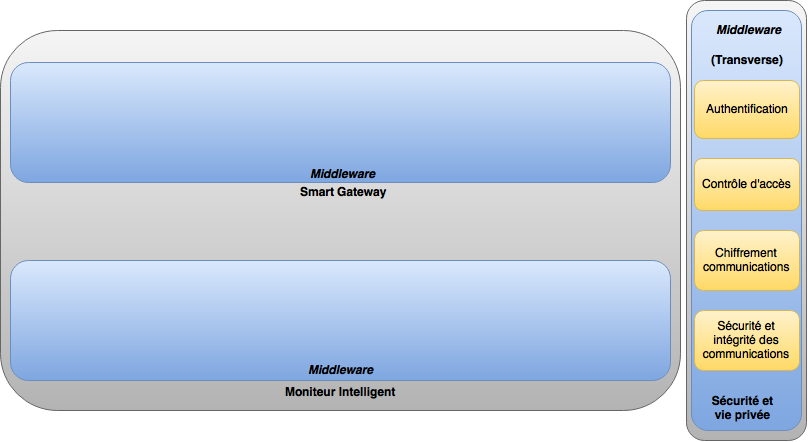
\includegraphics[width=1.5\textwidth]{Figure7.png}
	\caption{Modules de Sécurité et de Privacité dans le Middleware}
	\label{secu}
\end{figure}
\paragraph{}
Ainsi, nous avons conçu cette partie transverse du middleware afin de s'assurer d'une sécurité et d'une protection de la vie
privée maximale dans la limite des possibilités techniques. Les problématiques liées à la Qualité de Service (QoS) sont également
prises en compte par la vérification de l'intégrité, donc de la fiabilité des données transmises, afin d'éviter des situations potentiellement dangereuses.
